\subsection{Final solution on GitHub}\label{app:github}

The final solution along with the tutorial as well as this report are
on github: \url{https://github.com/niveK77pur/ExcaliburEnvironmentGCP}

\subsection{More on Markdown}\label{app:markdown}

An example of what the Markdown result looks like can be seen in
figure \ref{fig:markdown}

\subsubsection{Images}

The command we used to insert
images in the Markdown file is as follows.

\begin{verbatim}
<img src=Images/IMAGE_NAME.png width=1000>
\end{verbatim}

We used this html version instead of the default
\verb|![](Images/IMAGE_NAME.png)| because here you cannot specify a
size for the image. In Remarkable, the images were way too big and it
became quite unreadable, so we went with the html version since it
allows us to scale it to 1000 pixles in width.

\subsubsection{References}

Internal references need a tag to be
referenced. The tag and the reference look like this in Markdown.

\begin{verbatim}
	<a name=text-tag></a>
	Some text with a tag at the beginning.

	This is an [internal reference](#text-tag)
	while this is an
	[external reference](https://www.google.com)
\end{verbatim}

\begin{figure}
	\centering
	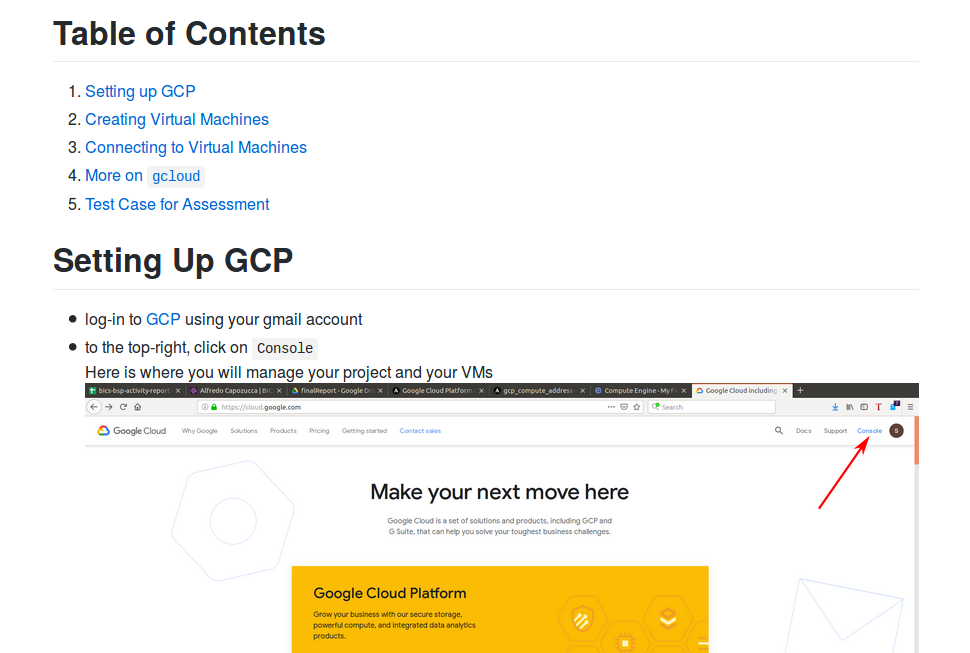
\includegraphics[width=.5\textwidth]{Images/markdown-showcase.png}
	\caption{Markdown example}
	\label{fig:markdown}
\end{figure}

